%\setcounter{chapter}{18}% Equivalent to "letter O"
%\renewcommand{\thechapter}{\Alph{chapter}}%

\chapter*{R\'esum\'e en fran\c{c}ais}
\addstarredchapter{R\'esum\'e en fran\c{c}ais}
\chaptermark{R\'esum\'e en fran\c{c}ais}

\minitoc

\section{Contexte et motivations}

Ce travail vise à explorer le formalisme port-Hamiltonien (pH) comme paradigme de modélisation, en particulier pour le cas des structures flexibles. Ce formalisme bénéficie de nombreuses propriétés intéressantes, car il fusionne intrinsèquement la géométrie avec la théorie des réseaux et du contrôle \cite{vanderschaft2006book}. Une caractéristique puissante de ce formalisme, en particulier pour la tâche de modélisation, est sa modularité. Les systèmes port-Hamiltonien (pHs) de dimension finie peuvent être facilement interconnectés entre eux \cite{cervera2007interconnection}. L'interconnexion est également possible dans le cas de dimension infinie \cite{kurula2010,augner2020int}. Finalement, il est également possible de coupler des systèmes de pH finis et infinis \cite{pasumarthy2006}. Cette fonctionnalité est particulièrement utile pour simplifier la tâche de modélisation dans les analyses préliminaires, ou, au contraire, pour réaliser des modèles haute fidélité de phénomènes multiphysiques complexes. \\

Le cadre port-Hamiltonien a été largement utilisé pour modéliser et contrôler des systèmes distribués issus de divers modèles physiques: les poutres de Timoshenko \cite{macchelli2004timo} et Euler-Bernoulli \cite{aoues2017modeling}, propagations d'ondes acoustiques \cite{trenchant2018}, réacteurs chimiques \cite{ramirez2013irreversible}, plasma dans les tomahawks \cite{vu2016plasma} et interactions fluide-structure \cite{cardoso2017}. La grande majorité de ces exemples se réfèrent à des modèles unidimensionnels. En effet, pour les systèmes pH linéaires unidimensionnels avec un opérateur anti-adjoint généralisé, \cite{legorrec2005} donne des conditions sur l'affectation des entrées et sorties aux limites pour que l'opérateur système génère un semi-groupe de contraction. Ce résultat a été largement utilisé pour construire des contrôleurs de frontière passifs pour les systèmes hyperboliques \cite{villegas2009exponential,macchelli2016synthesis,macchelli2020exponential}. \\

Depuis leur introduction, les systèmes port-Hamiltoniens distribués (dpH) ont été définis sur des domaines spatiaux multidimensionnels en utilisant le langage des formes différentielles \cite{vanderschaft2002}. Dans \cite{villegas2007}, la modélisation pH et l'approche en semi-groupe de systèmes à dimension infinie sont fusionnées. Ici, le cas des domaines multidimensionnels n'est que brièvement discuté. De nombreux autres exemples de pH sur des domaines multidimensionnels sont détaillés dans \cite[Chapitre 4]{duindam2009}. Cependant, les résultats d'existence et unicité n'y sont pas présentés. Une première contribution en ce sens peut être trouvée dans \cite{zwart2015wave}, où les auteurs démontrent l'existence et unicité de l'équation d'onde linéaire dans des dimensions géométriques arbitraires. Le récent article \cite{skrepek2019wellposedness} généralise ce résultat pour traiter le cas des pH linéaires génériques du premier ordre dans des dimensions géométriques arbitraires. Malgré toute cette littérature préexistante, les modèles issus de la mécanique structurale sur des domaines multidimensionnels n'ont quasiment jamais été considérés (à l'exception notable de \cite{macchelli2005mindlin} pour la modélisation de la plaque de Mindlin). \\

Le potentiel du cadre de pH comme paradigme de modélisation a été récemment exploré par les chercheurs. Par exemple, dans \cite{egger2018damped}, les auteurs considèrent un modèle port-Hamiltonien pour la propagation des ondes de pression dans les réseaux de tuyaux. En employant un schéma d'éléments finis mixtes, les auteurs réalisent une discrétisation préservant la structure du modèle d'origine. Un algorithme de réduction de modèle pour ce modèle discrétisé de réseau de pipelines est ensuite discuté dans \cite{egger2018}. Ces travaux récents confirment la validité de ce cadre pour aborder des scénarios d'application complexes et soulignent l'importance des algorithmes de discrétisation préservant la structure. Disposer de méthodologies capables de construire des discrétisations fiables est important non seulement pour la simulation, mais aussi à des fins de contrôle. En particulier, dans \cite{toledo2020}, les auteurs développent une méthode de synthèse systématique pour la conception de contrôleurs-observateurs pour le contrôle frontière des pHs sur des domaines spatiaux unidimensionnels. Pour construire l'observateur, une version discrétisée appropriée du système est supposée disponible. \\

Cette thèse tente d'établir un lien clair entre les modèles de mécanique structurale linéaire et les systèmes port-Hamiltoniens, à la fois pour les tâches de modélisation et de discrétisation. Ces deux finalités sont en effet fortement liées dans le contexte des pH. Pour obtenir une formulation de pH pour les modèles d'élasticité, il faut introduire la variable d'effort, associée à l'énergie de déformation, comme inconnue principale supplémentaire. Ajouter la variable de contrainte comme inconnue est le point de départ des éléments finis mixtes \cite{arnold1990intro}. Cela conduit à la décomposition de l'opérateur elliptique initial (c'est-à-dire le Laplacien ou bi-Laplacien), en deux opérateurs formellement adjoints. Par conséquent, la dynamique est régulée par un opérateur adjoint formellement antisymétrique, conduisant ainsi à un système Hamiltonien. Après avoir effectué une intégration par parties, une discrétisation mixte est immédiatement réalisée \cite{joly2003variational}. Ce raisonnement très concis élucide de manière informelle le lien étroit entre la modélisation port-Hamiltonienne de la mécanique des milieux continuum et les éléments finis mixtes.

\section{Plan de la thèse}

L'organigramme de la thèse est illustré sur la Fig. \ref{fig:organigramme}. La thèse est divisée en quatre parties principales.

\paragraph{Partie I (Chapitres 1, 2)}
Cette partie donne une introduction générale des travaux suivants. Le chapitre \ref{ch:reminder} rappelle brièvement ce que sont les systèmes pH de dimension finie ou infinie et comment ces systèmes sont profondément liés à la structure géométrique de Dirac ou de Stokes-Dirac (pour le cas de dimension finie et infinie respectivement).

\paragraph{Partie II (Chapitres 3, 4, 5)}
Cette partie est consacrée à la formulation de modèles appropriés d'élasticité et de thermoélasticité. Cette partie est subdivisée en trois chapitres.
\begin{itemize}
\item Le chapitre \ref{ch:elasPH} détaille la formulation du pH pour l'élasticité linéaire n-D générale.
\item Une formulation de pH de modèles de plaques minces (Kirchhoff-Love) et épaisses (Mindlin-Reissner) est donnée dans le chapitre \ref{ch:platePH}.
\item Le problème thermoélastique linéaire entièrement couplé est modélisé comme un système de pH couplé dans le chapitre \ref{ch:Thermo}.
\end{itemize}


\paragraph{Partie III (Chapitres 6, 7, 8)}
Cette partie est consacrée à la discussion et à l'implémentation du principal outil de discrétisation: la méthode des éléments finis partitionnés (PFEM). Cette méthode est une extension naturelle des éléments finis mixtes pour la discrétisation des pH. Cette partie se compose de trois chapitres.
\begin{itemize}
\item Une description détaillée du principe de fonctionnement de PFEM est donnée au chapitre \ref{ch:pfem}. Les bases d'approximation de cette discrétisation ne sont pas explicitement définies dans ce chapitre, car la méthode peut être implémentée en utilisant soit des éléments finis, soit des méthodes spectrales.
\item Une étude de convergence de plusieurs éléments finis est illustrée au chapitre \ref{ch:conv} pour le flexion de structures minces (poutres et plaques). Il ne s'agit en aucun cas d'une analyse mathématique rigoureuse de la convergence. Cependant, grâce à des résultats préexistants dans la littérature, les estimations d'erreur sont conjecturées et validées par des expériences numériques.
\item Le chapitre \ref{ch:applications} est dédié aux applications de la méthode PFEM. En particulier, l'accent est mis sur la stabilisation par injection d'amortissement, l'application des conditions aux limites mixtes et la validation du modèle pH thermoélastique pour une solution analytique.
\end{itemize}

\paragraph {Partie IV (Chapitres 9, 10)}
Dans cette partie, une formulation pH de systèmes multi-corps flexibles est discutée et validée. Le chapitre \ref{ch:fmdPH} détaille la dérivation d'un système pH associé à un corps flottant flexible sous l'hypothèse d'une petite déformation. Plusieurs applications sont alors considérées dans le chapitre \ref{ch:valid}.


\begin{sidewaysfigure}
\centering
\includegraphics[width=0.95\columnwidth]{part_1/scheme_outline.eps}%
\caption[]{Organigramme de la thèse.}%
\label{fig:organigramme}%
\end{sidewaysfigure}

\section{Mod\'elisation port-Hamiltonien des structures flexibles}
Dans cette section, un résumé concis des résultats concernant la modélisation de l'élasticité et la thermoélasticité linéaire est reporté. Une tractation détaillé peut être retrouvée dans les chapitres \ref{ch:elasPH}, \ref{ch:platePH} et \ref{ch:Thermo}


\subsection*{L'élasticité linéaire comme système port-Hamiltonien}

Dans cette section, une formulation port-Hamiltonienne de l'élasticité est déduite du problème classique d'élastodynamique. Il faut souligner que déjà dans les années soixante-dix une formulation purement hyperbolique de l'élasticité a été détaillée \cite{hughes1978classical}. Le point manquant est le lien clair avec la théorie des EDP Hamiltoniens. Une formulation Hamiltonienne peut être trouvée dans \cite[Chapitre 16]{grinfield2015}, mais sans aucun lien avec le concept de structure de Stokes-Dirac induit par la géométrie sous-jacente. \\

\paragraph{Variables d'énergie et de co-énergie}
Considérons un ensemble ouvert connecté $\Omega \subset \mathbb{R}^d, \; d \in \{2,3 \} $. Dans le cadre de l'élasticité linéaire, le déplacement dans un continuum déformable est donné par
\begin{equation*}
\rho \diffp[2]{\bm{u}}{t} - \Div(\bm{\mathcal{D}} \Grad \bm{u}) = 0, \qquad \bm{x} \in \Omega.
\end{equation*}
où $\rho$ est la densité et $\bm{\mathcal{D}}$ est le tenseur de rigidité (cf. Eq. \ref{eq:stiff3D}). Les opérateurs différentielles $\Div, \; \Grad$ sont définis dans l'appendice \ref{app:math}. Pour dériver une formulation pH, l'énergie totale, qui comprend l'énergie cinétique et de déformation, est nécessaire
\begin{equation*}
	H = \energy {\rho \norm{\partial_t \bm{u}}^2 + \bm{\Sigma} \cddot \bm{\varepsilon}}.
\end{equation*}
La notation $ \bm{A} \cddot \bm{B} = \Tr (\bm{A}^\top \bm{B}) = \sum_{i, j} A_{ij} B_{ij} $ désigne la contraction des tenseurs. Souvenez-vous que $\bm{\varepsilon} = \Grad {\bm{u}} $ et $ \bm{\Sigma} = \bm{\mathcal{D}} \bm{\varepsilon}$. Les variables d'énergie sont alors l'impulsion linéaire et le champ de déformation
\begin{equation*}
\bm{\alpha}_v = \rho \bm{v}, \qquad \bm{A}_{\varepsilon} = \bm{\varepsilon},
\end{equation*}
où $ \bm{v}: = \partial_t \bm{u}$. L'Hamiltonien peut être réécrit comme une fonctionnelle quadratique dans les variables d'énergie
\begin{equation*}
H = \energy{\frac{1}{\rho} \norm{\bm{\alpha}_v}^2 + (\bm{\mathcal{D}} \bm{A}_{\varepsilon}) \cddot \bm{A}_{\varepsilon}}.
\end{equation*}
Les variables de co-énergie sont données par
\begin{equation*}
\bm{e}_v: = \diffd{H}{\bm{\alpha}_v} = \bm{v}, \qquad \bm{E}_\varepsilon: = \diffd{H}{\bm{A}_{\varepsilon}} = \bm{\Sigma}.
\end{equation*}

\paragraph{Formulation port-Hamiltonien finale}
Il est maintenant possible d'expliciter la forme pH du système

\begin{equation*}
\diffp{}{t}
\begin{pmatrix}
\bm{\alpha}_v \\
\bm{A}_\varepsilon
\end{pmatrix} = 
\begin{bmatrix}
\bm{0} & \Div \\
\Grad & \bm{0} \\
\end{bmatrix}
\begin{pmatrix}
\bm{e}_v \\
\bm{E}_\varepsilon
\end{pmatrix}.
\end{equation*}
La première équation du système est la conservation du moment linéaire. Le second représente une condition de compatibilité. Le théorème \ref{th:adjDiv} assure que l'opérateur différentiel est formellement anti-adjoint (on peut également trouver ce résultat dans \cite[Lemme 3.3] {pauly2020elasticity}, disponible sous la forme de pré-impression arXiv). \\

Les variables aux bord sont ensuite trouvées en évaluant le bilan de puissance
\begin{equation*}
\begin{aligned}
\dot{H} &= \int_{\Omega} \left\{ \bm{e}_v \cdot \partial_t \bm\alpha_v + \bm{E}_\varepsilon \cddot \partial_t \bm{A}_\varepsilon \right\} \d\Omega, \\
&= \int_{\Omega} \left\{\bm{e}_v \cdot \Div \bm{E}_\varepsilon + \bm{E}_\varepsilon \cddot \Grad \bm{e}_v \right\}\d\Omega,\\
&= \int_{\Omega} \div(\bm{E}_\varepsilon \, \bm{e}_v) \d\Omega, \qquad \text{Théorème de Stokes (voir  Appendix \ref{app:math} Eq. \eqref{eq:intbypartsSymTens}}), \\
&= \int_{\partial \Omega} \bm{e}_v \cdot (\bm{E}_\varepsilon\bm{n}) \d{S} = \inner[L^2(\partial\Omega, \bbR^d)]{\bm{e}_v}{\bm{E}_\varepsilon \, \bm{n}}.
\end{aligned}
\end{equation*}

L'imposition du champ de vitesse le long de la frontière $ \bm{e}_v = \partial_t \bm{u} $ correspond à une condition de Dirichlet. Si c'est la traction a être imposée $ \bm{E}_\varepsilon \, \bm{n} = \bm{\Sigma} \, \bm{n} = \bm{t}$, on a une condition de Neumann. Considérons une partition de la frontière $\partial \Omega = \overline{\Gamma}_N \cup \overline{\Gamma}_D $ et $\Gamma_N \cap \Gamma_D = \{\emptyset\} $, où une condition de Dirichlet et une de Neumann s'appliquent respectivement au sous-ensemble ouvert $\Gamma_D $ et $\Gamma_N $ (voir Fig. \ref{fig:bc_elas2D}). Ensuite, la formulation pH finale devient

\begin{equation*}
\begin{aligned}
\displaystyle
\diffp{}{t}
\begin{pmatrix}
\bm{\alpha}_v \\
\bm{A}_\varepsilon
\end{pmatrix} &= \underbrace{
	\begin{bmatrix}
	\bm{0} & \Div \\
	\Grad & \bm{0} \\
	\end{bmatrix}}_{\mathcal{J}}
\begin{pmatrix}
\bm{e}_v \\
\bm{E}_\varepsilon
\end{pmatrix}, \vspace{3pt}\\
\bm{u}_\partial &= \underbrace{
	\begin{bmatrix}
	\bm\gamma_{0}^{\Gamma_D} & \bm{0} \\
	\bm{0} & \bm\gamma_n^{\Gamma_N} \\
	\end{bmatrix}}_{\mathcal{B}_\partial} \begin{pmatrix}
\bm{e}_v \\
\bm{E}_\varepsilon
\end{pmatrix}, \qquad
\bm{y}_\partial = \underbrace{
	\begin{bmatrix}
	\bm{0} & \bm\gamma_{n}^{\Gamma_D} \\
	\bm\gamma_0^{\Gamma_N} & \bm{0} \\
	\end{bmatrix}}_{\mathcal{C}_\partial}
\begin{pmatrix}
\bm{e}_v \\
\bm{E}_\varepsilon
\end{pmatrix},
\end{aligned}
\end{equation*}
où $\bm\gamma_{0}^{\Gamma_*}$ désigne la trace sur l'ensemble $\Gamma_* $, soit $ \bm\gamma_{0}^{\Gamma_*} \bm{e}_v = \bm{e}_v \vert_{\Gamma_*} $. De plus, $ \bm\gamma_{n}^{\Gamma_*} $ désigne la trace normale sur l'ensemble $\Gamma_*$, à savoir $\bm\gamma_{n}^{\Gamma_*} \bm{E}_\varepsilon = \bm{E}_\varepsilon \bm{n} \vert_{\Gamma_*}$. Les opérateurs de frontière $\mathcal{B}_\partial, \mathcal{C}_\partial $ sont non bornés.

\subsection*{Le modèles de plaques en forme port-Hamiltonien}
Dans cette section on résume les modèles port-Hamiltonien de plaques minces. On s'intéresse en particulier aux modèles dus à Mindlin \cite{mindlin1951} et Kirchhoff. 

\paragraph{Plaque de Mindlin}
Ce modèle décrit les déformations des plaques modérément épaisses, i.e. le rapport entre l'épaisseur et la longueur est de l'ordre de $10^{-1}$. Le système finale est donné par 2 EDP couplées ayant comme inconnus le déplacement vertical $w$ et la rotation $\bm{\theta}$ des segment perpendiculaire à la surface non déformée (pour les détails de calculs voir \cite[Chapter 10]{reddy2006theory})
\begin{equation*}
\begin{aligned}
\rho h \diffp[2]{w}{t} &= \div \bm{q}, \qquad (x,y) \in \Omega, \\
\frac{\rho h^3}{12} \diffp[2]{\bm{\theta}}{t} &=\Div \bm{M} + \bm{q},
\end{aligned}
\end{equation*}
où $h$ est l'épaisseur, $\bm{M}= \bm{\mathcal{D}}_b\,\Grad{\bm{\theta}}$ et $\bm{q}= K_{\text{sh}} Gh\,(\grad w - \bm{\theta})$. $\Omega \subset \mathbb{R}^2$ est un domaine connecté et borné. Le tenseur de rigidité à flexion $\bm{\mathcal{D}}_b$ est donné, dans la cas d'un matériel isotrope, par l'Eq. \eqref{eq:Db}. $K_{\text{sh}}$ est le facteur correctif du au cisaillement et $G$ le module du cisaillement.

Considérons l'Hamiltonien (énergie totale)
\begin{equation*}
H = \frac{1}{2} \int_{\Omega}  \left\{ \rho h \left(\diffp{w}{t} \right)^2 + \frac{\rho h^3}{12} \norm{\diffp{\bm{\theta}}{t}}^2 +   \bm{M} \cddot \bm{\kappa} + \bm{q} \cdot \bm{\gamma}  \right\}  \d\Omega, 
\end{equation*}
où $\bm{\kappa} = \Grad \bm{\theta}, \; \bm{\gamma} = \grad w - \bm{\theta}$. Le choix des variables d'énergie est le même que dans \cite{macchelli2005mindlin} mais ici des variables scalaires, vectorielles et tensorielles sont regroupées:
\begin{equation*}
\begin{aligned}
\alpha_w &= \rho h \diffp{w}{t}, \quad &\text{Moment linéaire,} \\
\bm{A}_{\kappa} &= \bm{\kappa}, \quad &\text{Tenseur de courbure,} \\
\end{aligned} \qquad
\begin{aligned}
\bm\alpha_{\theta} &=  \frac{\rho h^3}{12} \diffp{\bm{\theta}}{t}, \quad &\text{Moment angulaire,}\\
\bm\alpha_{\gamma} &= \bm{\gamma}. \quad &\text{Deformation au cisaillement.}\\
\end{aligned}
\end{equation*}
L'Hamiltonien est maintenant un fonctionnelle quadratique dans les variables d'énergies
\begin{equation*}
H = \frac{1}{2} \int_{\Omega}  \left\{ \frac{1}{\rho h}\alpha_w^2 + \frac{12}{\rho h^3} \norm{\bm{\alpha}_{\theta}}^2 + (\bm{\mathcal{D}}_b \bm{A}_\kappa) \cddot \bm{A}_\kappa + (\bm{\mathcal{D}}_s \bm{\alpha}_\gamma) \cdot  \bm{\alpha}_\gamma  \right\}  \d\Omega, 
\end{equation*}
Les variables de co-énergie sont trouvées en calculant la dérivée variationnelle de l'Hamiltonien:
\begin{equation*}
\begin{aligned}
e_w &:= \diffd{H}{\alpha_w} = \diffp{w}{t},  \quad &\text{Vitesse linéaire,} \\
\bm{E}_{\kappa} &:= \diffd{H}{\bm{A}_{\kappa}} = \bm{M}, \quad &\text{Tenseur de moments,}\\
\end{aligned} \qquad
\begin{aligned}
\bm{e}_{\theta} &:= \diffd{H}{\bm\alpha_{\theta}} = \diffp{\bm{\theta}}{t}, \quad &\text{Vitesse angulaire,}  \\
\bm{e}_{\gamma} &:= \diffd{H}{\bm\alpha_{\gamma}} = \bm{q} \quad &\text{Effort tranchant.} \\
\end{aligned}
\end{equation*}
Une fois les variables concaténées, le système pH est exprimé comme suit
\begin{equation*}
\diffp{}{t}
\begin{pmatrix}
\alpha_w \\
\bm\alpha_\theta \\
\bm{A}_\kappa \\
\bm\alpha_{\gamma} \\
\end{pmatrix} = 
\begin{bmatrix}
0  & 0  & 0  & \div \\
\bm{0} & \bm{0} &  \Div & \bm{I}_{2 \times 2}\\
\bm{0}  & \Grad  & \bm{0}  & \bm{0}\\
\grad & -\bm{I}_{2 \times 2} &  \bm{0} & \bm{0} \\
\end{bmatrix}
\begin{pmatrix}
e_w \\
\bm{e}_{\theta} \\
\bm{E}_{\kappa} \\
\bm{e}_{\gamma} \\
\end{pmatrix}.
\end{equation*}
Nous allons maintenant établir le bilan énergétique total en termes de variables au bord car elles feront partie de la structure de Stokes-Dirac sous-jacente de ce modèle. Le bilan de puissance devient
\begin{equation*}
\dot{H}= \int_{\partial \Omega} \left\{ w_t \, q_n  + \omega_n \, M_{nn} + \omega_s \, M_{ns} \right\} \d{s},  
\end{equation*}
Le résultat est obtenu en appliquant le théorème de Stokes. Les variables au bord (illustrées dans la Fig.~\ref{fig:Cauchy_law}) sont définies comme suit:
\begin{equation*}
\begin{aligned}
\text{Effort de cisaillement}  \qquad q_{n} &:= \bm{q} \cdot \bm{n}=  \bm{e}_{\gamma} \cdot \bm{n},  \\
\text{Moment de flexion} \quad 
M_{nn} &:=  \bm{M} \cddot (\bm{n}\otimes{\bm{n}}) = \bm{E}_{\kappa} \cddot (\bm{n}\otimes{\bm{n}}), 	\\
\text{Moment de torsion} \quad M_{ns} &:= \bm{M} \cddot (\bm{s}\otimes{\bm{n}}) = \bm{E}_{\kappa} \cddot (\bm{s}\otimes{\bm{n}}),	
\end{aligned}
\end{equation*}

Étant donné deux vecteurs $\bm{a} \in \mathbb{R}^n, \, \bm{b} \in \mathbb{R}^m $, la notation $ \bm{a} \otimes {\bm{b}} = \bm{a} \bm{b}^\top \in \mathbb{R}^{n \times m} $ désigne le produit extérieur (ou dyadique) de deux vecteurs. Les vecteurs $\bm{n} $ et $ \bm{s}$ désignent les vecteurs unitaires normaux et tangentiels à la frontière, comme le montre la Fig. \ref{fig:plate_ref}. Les variables conjuguées au sens de la puissance sont
\begin{equation*} 
\begin{aligned}
\text{Vitesse verticale}  \quad w_t &:= \diffp{w}{t} = e_w, \\
\text{Rotation en flexion} \quad 
\omega_{n} &:= \diffp{\bm{\theta}}{t} \cdot \bm{n} = \bm{e}_\theta \cdot \bm{n} \\
\text{Rotation en torsion} \quad 
\omega_{s} &:= \diffp{\bm{\theta}}{t} \cdot \bm{s} = \bm{e}_\theta \cdot \bm{s}.	
\end{aligned},
\end{equation*}
Considérons une partition de la frontière $\partial\Omega = \overline{\Gamma}_{C} \cup \overline {\Gamma}_{S} \cup \overline {\Gamma}_{F}, \; {\Gamma}_{C} \cap{\Gamma}_{S} \cap {\Gamma}_{F} = \{\emptyset\} $. Le sous-ensemble ouvert $\Gamma_{C}, \, \Gamma_{S}, \, \Gamma_{F} $ peut être vide. Les conditions aux limites de la plaque Mindlin \cite{duran1999approximation} (voir Fig. \ref{fig:bcs_min}) qui sont considérées sont:
\begin{itemize}
\item Encastrement (C) sur $\Gamma_{C} \subseteq \partial \Omega $: $ w_t, \ \omega_{n}, \ \omega_{s}$ connus;
\item Bord simplement appuyé  (S) sur $\Gamma_{S} \subseteq \partial \Omega $: $ w_t, \ \omega_{s}, \ M_{nn} $ connus;
\item  Bord libre (F) sur $ \Gamma_{F} \subseteq \partial \Omega $: $ M_{nn}, \ M_{ns}, \ q_n$ connus.
\end{itemize}
Ensuite, la formulation finale du pH devient
\begin{equation*}
\begin{aligned}
\displaystyle
\diffp{}{t}
\begin{pmatrix}
\alpha_w \\
\bm\alpha_\theta \\
\bm{A}_\kappa \\
\bm\alpha_{\gamma} \\
\end{pmatrix} &= 
\underbrace{\begin{bmatrix}
	0  & 0  & 0  & \div \\
	\bm{0} & \bm{0} &  \Div & \bm{I}_{2 \times 2}\\
	\bm{0}  & \Grad  & \bm{0}  & \bm{0}\\
	\grad & -\bm{I}_{2 \times 2} &  \bm{0} & \bm{0} \\
	\end{bmatrix}}_{\mathcal{J}}
\begin{pmatrix}
e_w \\
\bm{e}_{\theta} \\
\bm{E}_{\kappa} \\
\bm{e}_{\gamma} \\
\end{pmatrix}, \vspace{3pt}\\
\bm{u}_\partial &= \underbrace{
	\begin{bmatrix}
	\gamma_{0}^{\Gamma_C} & {0} & {0} & {0} \\
	{0} & \gamma_n^{\Gamma_C} &  {0} & {0} \\
	{0} & \gamma_s^{\Gamma_C} &  {0} & {0} \\
	\gamma_{0}^{\Gamma_S} & {0} & {0} & {0} \\
	{0} & \gamma_s^{\Gamma_S} & {0} & {0} \\
	{0} &  {0} & \gamma_{nn}^{\Gamma_S} & {0} \\
	{0} &  {0} & \gamma_{nn}^{\Gamma_F} & {0} \\
	{0} &  {0} & \gamma_{ns}^{\Gamma_F} & {0} \\
	{0} &  {0} & {0} & \gamma_{n}^{\Gamma_F} \\
	\end{bmatrix}}_{\mathcal{B}_\partial} \begin{pmatrix}
e_w \\
\bm{e}_{\theta} \\
\bm{E}_{\kappa} \\
\bm{e}_{\gamma} \\
\end{pmatrix}, \vspace{3pt}\qquad
\bm{y}_\partial = \underbrace{
	\begin{bmatrix}
	{0} & {0} & {0} & \gamma_{n}^{\Gamma_C} \\
	{0} & {0} & \gamma_{nn}^{\Gamma_C} & {0} \\
	{0} & {0} & \gamma_{ns}^{\Gamma_C} & {0} \\
	{0} & {0} & {0} & \gamma_{n}^{\Gamma_S} \\
	{0} & {0} & \gamma_{ns}^{\Gamma_S} & {0} \\
	{0} & \gamma_{n}^{\Gamma_S} & {0} & {0} \\
	{0} & \gamma_{n}^{\Gamma_F} & {0} & {0} \\
	{0} & \gamma_{s}^{\Gamma_F} & {0} & {0} \\
	\gamma_{0}^{\Gamma_F} & {0} & {0} & {0} \\
	\end{bmatrix}}_{\mathcal{C}_\partial}
\begin{pmatrix}
e_w \\
\bm{e}_{\theta} \\
\bm{E}_{\kappa} \\
\bm{e}_{\gamma} \\
\end{pmatrix},
\end{aligned}
\end{equation*}
où $\gamma_{0}^{\Gamma_*} a = a \vert_{\Gamma_*} $ désigne la trace sur l'ensemble $\Gamma_*$. De plus, les notations $\gamma_{n}^{\Gamma_*} \bm{a} = \bm{a} \cdot \bm{n} \vert_{\Gamma_*}, \, \gamma_{s}^{\Gamma_*} \bm{a} = \bm{a} \cdot \bm{s} \vert_{\Gamma_*} $ indiquent respectivement les traces normales et tangentielles sur l'ensemble $\Gamma_* $. Les symboles $\gamma_{nn}^{\Gamma_*}, \gamma_{ns}^{\Gamma_*} $ désignent la trace normale-normale et la trace normale-tangentielle des fonctions tensorielles et $ \gamma_{nn}^{\Gamma_*} \bm{A} = \bm{A} \cddot (\bm{n} \otimes \bm{n}) \vert_{\Gamma_*}, \, \gamma_{ns}^{\Gamma_*} \bm{A} = \bm{A} \cddot (\bm{n} \otimes \bm{s}) \vert_{\Gamma_*} $. 

\paragraph{Plaque de Kirchhoff}
Le modèle de Kirchhoff corresponds à une EDP scalaire qui décrit l'évolution du déplacement verticale pour des plaques minces (rapport entre épaisseur et longueur de l'ordre de $10^{-3}$). Le modèle peut être dérivée en utilisant le principe de Hamilton et est donné par l'équation suivante (pour les calculs détaillés, le lecteur peut consulter \cite[Chapter 3]{reddy2006theory})
\begin{equation*}
\rho h \diffp[2]{w}{t} = - \div\Div (\bm{\mathcal{D}}_b\, \Grad\grad{w}), \qquad (x,y) \in \Omega.
\end{equation*}

Encore une fois, le point de départ pour obtenir une formulation port-Hamiltonien est l'Hamiltonien (énergie totale)
\begin{equation*}
H = \frac{1}{2} \int_{\Omega} \left\{\rho h \left(\diffp{w}{t} \right)^2 + \bm{M} \cddot \bm{\kappa}  \right\}  \d{\Omega},
\end{equation*}
où $ \bm{\kappa} = \Grad\grad{w}, \; \bm{M} = \bm{\mathcal{D}}_b \Grad\grad{w}$. Pour ce qui concerne le choix des variables d'énergie, une variable scalaire et une tensorielle sont considérés:
\begin{equation*}
\alpha_w = \rho h \diffp{w}{t}, \quad \text{Moment linéaire}, \qquad \bm{A}_{\kappa} = \bm{\kappa}, \quad \text{Tenseur de corbure}.	
\end{equation*}
Les variables de co-énergie sont trouvées en calculant la dérivée variationnelle de l'Hamiltonien:
\begin{equation*}
e_w := \diffd{H}{\alpha_w} = \diffp{w}{t}, \quad \text{Vitesse linéaire},  \qquad  \bm{E}_{\kappa} := \diffd{H}{\bm{A}_{\kappa}} = \bm{M}, \quad \text{Tenseur de moment}.
\end{equation*}

Le système port-Hamiltonien associé s'écrit de la manière suivante
\begin{equation*}
\diffp{}{t}
\begin{pmatrix}
\alpha_w \\
\bm{A}_{\kappa} \\
\end{pmatrix} = 
\begin{bmatrix}
0  &  - \div \circ \Div \\
\Grad \circ \grad & \bm{0} \\
\end{bmatrix}
\begin{pmatrix}
e_w \\
\bm{E}_{\kappa} \\
\end{pmatrix}.
\end{equation*}
La première équation représente la dynamique, la seconde le fait que les dérivés d'ordre supérieur commutent. Le théorème \ref{th:adjdivDiv} assure que l'opérateur qui régis la dynamique est anti-symétrique. Le bilan de puissance fournit les variables au bord
\begin{equation*}
\dot{H} = \int_{\partial \Omega} \left\{ w_t \, \widetilde{q}_n + \partial_{\bm{n}}{w_t} \, M_{nn}\right\} \, \d{s}, 
\end{equation*} 
Les variables au bord sont définis 
\begin{equation*}
	\begin{aligned}
	\text{Effort de cisaillement}  \qquad \widetilde{q}_{n} &:= - \bm{n} \cdot \mathrm{Div}(\bm{E}_{\kappa}) - \partial_{\bm{s}}{M_{ns}}, \\
	\text{Moment de flexion} \quad M_{nn} &:=  \bm{M} \cddot (\bm{n}\otimes{\bm{n}}) = \bm{E}_{\kappa} \cddot (\bm{n}\otimes{\bm{n}}),
	\end{aligned}
\end{equation*}
Les variables conjuguées au sens de la puissance sont données par
\begin{equation*}
	\begin{aligned}
	\text{Vitesse verticale}  \qquad w_t &:= \diffp{w}{t} = e_w, \\
	\text{Rotation en flexion} \quad 
	\partial_{\bm{n}}{w_t} &:= \nabla{e_w} \cdot \bm{n}.
	\end{aligned},
\end{equation*}
Considérons une partition de la frontière $ \partial \Omega = \overline{\Gamma}_{C} \cup \overline{\Gamma}_{S} \cup \overline {\Gamma}_{F}, \; {\Gamma}_{C} \cap {\Gamma}_{S} \cap {\Gamma}_{F} = \{\emptyset\} $, où $ {\Gamma}_{C}, {\Gamma}_{S}, {\Gamma}_{F} $ sont un sous-ensemble ouvert de $\partial \Omega $. Les conditions aux limites pour la plaque de Kirchhoff \cite{gustafsson2018} sont les suivantes (voir Fig. \ref{fig:bcs_kirchh}):
\begin{itemize}
\item Encastrée (C) sur $ \Gamma_{C} \subseteq \partial \Omega $: $ w_t, \ \partial_{\bm{n}} {w_t} $ connu;
\item Appui simple (S) sur $ \Gamma_{S} \subseteq \partial\Omega $: $ w_t, \ M_{nn} $ connu;
\item Libre (F) sur $ \Gamma_{F} \subseteq \partial \Omega $: $ \widetilde {q}_n, \ M_{nn} $ connu.
\end{itemize}
Ensuite, la formulation finale du pH devient
\begin{equation*}
\begin{aligned}
\displaystyle
\diffp{}{t}
\begin{pmatrix}
\alpha_w \\
\bm{A}_{\kappa} \\
\end{pmatrix} &= 
\underbrace{\begin{bmatrix}
	0  &  - \div \circ \Div \\
	\Grad \circ \grad & \bm{0} \\
	\end{bmatrix}}_{\mathcal{J}}
\begin{pmatrix}
e_w \\
\bm{E}_{\kappa} \\
\end{pmatrix}, \vspace{3pt}\\
\bm{u}_\partial &= \underbrace{
	\begin{bmatrix}
	\gamma_{0}^{\Gamma_C} & {0}  \\
	\gamma_1^{\Gamma_C} &  {0} \\
	\gamma_{0}^{\Gamma_S} &  {0}  \\
	{0} & \gamma_{nn}^{\Gamma_S} \\
	{0} & \gamma_{nn, 1}^{\Gamma_F}  \\
	{0} & \gamma_{nn}^{\Gamma_F}\\
	\end{bmatrix}}_{\mathcal{B}_\partial} \begin{pmatrix}
e_w \\
\bm{E}_{\kappa} \\
\end{pmatrix},\qquad
\bm{y}_\partial = \underbrace{
	\begin{bmatrix}
	{0} & \gamma_{nn, 1}^{\Gamma_C} \\
	{0} & \gamma_{nn}^{\Gamma_C} \\
	{0} & \gamma_{nn, 1}^{\Gamma_S} \\
	\gamma_{1}^{\Gamma_S} & {0} \\
	\gamma_{0}^{\Gamma_F} & {0} \\
	\gamma_{1}^{\Gamma_F} & {0} \\
	\end{bmatrix}}_{\mathcal{C}_\partial}
\begin{pmatrix}
e_w \\
\bm{E}_{\kappa} \\
\end{pmatrix},
\end{aligned}
\end{equation*}
où $ \gamma_{0}^{\Gamma_*} a = a \vert_{\Gamma_*} $ et $ \gamma_{1}^{\Gamma_*} a = \partial_{\bm{n}} a \vert_{\Gamma_*} $ désignent respectivement la trace et la trace dérivée normale sur l'ensemble $\Gamma_*$. Le symbole $\gamma_{nn, 1}^{\Gamma_*}$ désigne la trace $\gamma_{nn, 1}^{\Gamma_*} \bm{A} = -\bm{n} \cdot \Div \bm{A} - \partial_{\bm{s}} (\bm{A} \cddot (\bm{n} \otimes \bm{s})) \vert_{\Gamma_*}$, tandis que $\gamma_{nn}^{\Gamma_*} \bm{A} = \bm{A} \cddot (\bm{n} \otimes \bm{n}) \vert_{\Gamma_*} $ indique la  trace normale-normale d'une fonction tensorielle. 

\subsection*{Le problème thermoélastique linéaire couplé}
Pour les problèmes thermoélastiques linéaires, on s'aperçoit que les modèles classique peuvent être réécrits comme deux systèmes port-Hamiltonien couplés. Considérons à nouveau l'équation d'élasticité sur $\Omega \subset \mathbb{R}^d, \, d \ in \{1, 2, 3 \} $, avec une entrée distribuée $\bm{u}_E$ qui joue le rôle d'une force externe
\begin{equation*}
\begin{aligned}
\diffp{}{t}
\begin{pmatrix}
\bm{\alpha}_v \\
\bm{A}_{\varepsilon} \\
\end{pmatrix} &= 
\begin{bmatrix}
\bm{0} & \Div \\
\Grad & \bm{0} \\
\end{bmatrix}
\begin{pmatrix}
\bm{e}_v \\
\bm{E}_{\varepsilon} \\
\end{pmatrix} + 
\begin{bmatrix}
\bm{I}_{d\times d} \\
\bm{0} \\
\end{bmatrix}\bm{u}_E, \\
\bm{y}_E &= \begin{bmatrix}
\bm{I}_{d\times d} & \bm{0} \\
\end{bmatrix}
\begin{pmatrix}
\bm{e}_v \\
\bm{E}_{\varepsilon}
\end{pmatrix},
\end{aligned}
\end{equation*}
avec Hamiltonien
\[
H_E = \energy{\bm{\alpha}_v \cdot \bm{e}_v + \bm{A}_{\varepsilon} \cddot \bm{E}_{\varepsilon}}.
\]
L'équation de la chaleur admet la représentation différentielle-algébrique (pHDAE) suivante
\begin{equation*}
\begin{aligned}
\begin{bmatrix}
1 & 0 \\
\bm{0} & \bm{0} \\
\end{bmatrix}
\diffp{}{t}
\begin{pmatrix}
\alpha_T \\
\bm{j}_Q \\
\end{pmatrix} &= 
\begin{bmatrix}
0 & -\div \\
-\grad & -(T_0 k)^{-1} \\
\end{bmatrix}
\begin{pmatrix}
e_T \\
\bm{j}_Q \\
\end{pmatrix} + 
\begin{bmatrix}
1 \\
\bm{0} \\
\end{bmatrix} u_T, \\
y_T &= \begin{bmatrix}
1 & \bm{0} \\
\end{bmatrix} \begin{pmatrix}
e_T \\
\bm{j}_Q \\
\end{pmatrix},
\end{aligned}
\end{equation*} 
où les variables sont définies comme suit
\begin{equation*}
\alpha_T := \rho c_\epsilon (T-T_0), \qquad e_T := \frac{T-T_0}{T_0} =: \theta, \qquad \bm{j}_Q := -k \grad T.
\end{equation*}
Les paramètres $c_\epsilon, \; k, \; T_0$ sont la capacité thermique à déformation constante, le coefficient de diffusivité et une température de référence.
L'entrée $u_T$ joue le rôle d'une source de chaleur distribuée. L'Hamiltonien corresponds à une fonctionnelle quadratique (c'est n'est pas l'énergie interne)
\begin{equation*}
H_T = \frac{1}{2}\int_\Omega {e}_T {\alpha}_T \d\Omega.
\end{equation*}
Considérez l'interconnexion suivante
\begin{equation*}
\bm{u}_E = - \Div(\bm{\mathcal{C}}_\beta \, y_T), \qquad
u_T = - \bm{\mathcal{C}}_\beta \cddot\Grad(\bm{y}_E). 
\end{equation*}
où on a introduit l'opérateur de couplage
\[\bm{\mathcal{C}}_\beta:=T_0 \beta(2\mu + 3 \lambda)\bm{I}_{d\times d}, \]
avec $\beta$ le coefficient de dilatation thermique et $\lambda, \mu$ les coefficients de Lamé. L'interconnexion préserve l'énergie car elle peut être écrite de manière compacte comme
\begin{equation*}
\bm{u}_E = \mathcal{A}_\beta(y_T), \qquad u_T = - \mathcal{A}_\beta^*(\bm{y}_E), \where  \mathcal{A}_\beta(\cdot) = - \Div(\bm{\mathcal{C}}_\beta \, \cdot),
\end{equation*}
où $\mathcal{A}_\beta^*$ indique l'adjoint formelle. Le problème thermoélastique couplé peut maintenant être écrit comme
\begin{equation*}
\begin{bmatrix}
\bm{1} & \bm{0} & \bm{0} & \bm{0}\\
\bm{0} & \bm{1} & \bm{0} & \bm{0}\\
0 & 0 & 1 & 0\\
\bm{0} & \bm{0} & \bm{0} & \bm{0}\\
\end{bmatrix}
\diffp{}{t}
\begin{pmatrix}
\bm{\alpha}_v \\
\bm{A}_\varepsilon \\
{\alpha}_T \\
\bm{j}_Q \\
\end{pmatrix} = 
\begin{bmatrix}
\bm{0} & \Div & \mathcal{A}_\beta & \bm{0}\\
\Grad & \bm{0} & \bm{0} & \bm{0} \\
- \mathcal{A}_\beta^* & 0 & 0 & -\div \\
\bm{0} & \bm{0} & -\grad & - (T_0 k)^{-1} \\
\end{bmatrix}
\begin{pmatrix}
\bm{e}_v \\
\bm{E}_\varepsilon \\
{e}_T \\
\bm{j}_Q \\
\end{pmatrix},
\end{equation*}
Le bilan de puissance global est facilement calculé comme
\begin{equation*}
\begin{aligned}
\dot{H} = \dot{H}_E + \dot{H}_T \le \int_{\partial \Omega} \left\{\left[\bm{E}_\varepsilon - e_T \bm{\mathcal{C}}_\beta \right] \cdot \bm{n}\right\}  \cdot \bm{e}_v  \d{S} - \int_{\partial\Omega} e_T \ \bm{j}_Q \cdot \bm{n} \d{S}.
\end{aligned}
\end{equation*}
Le système finale et le bilan de puissance associé sont identique aux résultats reportés in \cite[page 326, 332]{carlson1973}. Soit une partition de la frontière $\partial \Omega = \Gamma_D^E \cup \Gamma_N^E = \Gamma_D^T \cup \Gamma_N^T$ pour le domaine élastique et thermique. Les conditions aux limites générales sont données par (voir Fig. \ref{fig:bc_TherElas2D})
\begin{equation*}
\begin{aligned}
\bm{e}_v \text{ connu sur } \Gamma_D^E \times (0, +\infty), \\
(\bm{E}_\varepsilon - \bm{\mathcal{C}}_\beta e_T) \cdot \bm{n} \text{ connu sur } \Gamma_N^E \times (0, +\infty), 
\end{aligned} \qquad
\begin{aligned}
e_T \text{ connu sur } \Gamma_D^T \times (0, +\infty), \\
\bm{j}_Q \cdot \bm{n} \text{ connu sur } \Gamma_N^T \times (0, +\infty).
\end{aligned}
\end{equation*}
À partir du bilan de puissance, les conditions aux limites classiques sont extraites. Cela permet de définir des opérateurs de frontière appropriés pour le problème thermoélastique
\begin{equation*}
\bm{u}_\partial = 
\underbrace{\begin{bmatrix}
	\bm{\gamma}_{0}^{\Gamma_D^E} & \bm{0} & \bm{0} & \bm{0} \\
	\bm{0} & \bm{\gamma}_n^{\Gamma_N^E} & - \bm{\gamma}_n^{\Gamma_N^E}(\bm{\mathcal{C}}_\beta\, \cdot )  & \bm{0}  \\ 
	{0} & {0} & {\gamma}_{0}^{\Gamma_D^T} & {0} \\
	\bm{0} & \bm{0} & \bm{0} & \bm{\gamma}_{n}^{\Gamma_N^T} \\
	\end{bmatrix}}_{\mathcal{B}_\partial}
\begin{pmatrix}
\bm{e}_v \\
\bm{E}_\varepsilon \\
{e}_T \\
\bm{j}_Q \\
\end{pmatrix}, \; 
\bm{y}_\partial = 
\underbrace{\begin{bmatrix}
	\bm{0} & \bm{\gamma}_n^{\Gamma_D^E} & - \bm{\gamma}_n^{\Gamma_D^E}(\bm{\mathcal{C}}_\beta\, \cdot )  & \bm{0}  \\ 
	\bm{\gamma}_{0}^{\Gamma_N^E} & \bm{0} & \bm{0} & \bm{0} \\
	\bm{0} & \bm{0} & \bm{0} & \bm{\gamma}_{n}^{\Gamma_D^T} \\
	{0} & {0} & {\gamma}_{0}^{\Gamma_N^T} & {0} \\
	\end{bmatrix}}_{\mathcal{C}_\partial}
\begin{pmatrix}
\bm{e}_v \\
\bm{E}_\varepsilon \\
{e}_T \\
\bm{j}_Q \\
\end{pmatrix}.
\end{equation*} 

\section{Développement de la méthode PFEM}
Une discrétisation préservant la structure est capable de construire un système de pH équivalent qui possède les propriétés structurelles du modèle d'origine:
\begin{tcbraster}[raster columns=2, raster equal height]
	\begin{tcolorbox}[width=0.4\textwidth, nobeforeafter, colframe=theme,title=Système pH de dimension infinie]%%
		EDP avec entrées distribuées:
		\begin{align*}
		\partial_t {\bm{\alpha}}(\bm{x}, t) &= \mathcal{J} {\displaystyle \delta_{\bm{\alpha}} {H}}+ \mathcal{B} \textcolor{red}{\bm{u}_\Omega(\bm{x}, t)}, \\
		\textcolor{red}{\bm{y}_\Omega(\bm{x}, t)} &= \mathcal{B}^* {\displaystyle  \delta_{\bm{\alpha}} {H}}.
		\end{align*}
		Conditions aux limites: 
		\[\textcolor{blue}{\bm{u}_\partial} = \mathcal{B}_\partial{\displaystyle  \delta_{\bm{\alpha}} {H}}, \quad \textcolor{blue}{\bm{y}_\partial} = \mathcal{C}_\partial {\displaystyle  \delta_{\bm{\alpha}} {H}}. \]
		Bilan de puissance (Théorème de Stokes): 
		\[ \dot{H} = \displaystyle \int_{\partial \Omega} \textcolor{blue}{\bm{u}_\partial} \cdot \textcolor{blue}{\bm{y}_\partial} \d{S} +  \int_{\Omega} \textcolor{red}{\bm{u}_\Omega} \cdot \textcolor{red}{\bm{y}_\Omega} \d{\Omega}.
		\]
	\end{tcolorbox} 
	\begin{tcolorbox}[width=0.4\textwidth, nobeforeafter,  colframe=theme,title=Discretisation préservant la structure]%%
		EDO résultante:
		\begin{align*}
		\dot{\bm{\alpha}}_d &= \mathbf{J} \, {\nabla {H}_d} + \mathbf{B}_\Omega \textcolor{red}{\mathbf{u}_\Omega} + \mathbf{B}_\partial \textcolor{blue}{\mathbf{u}_\partial}, \\
		\textcolor{red}{\mathbf{y}_\Omega} &= \mathbf{B}_\Omega^\top \, {\nabla {H}_d}, \\
		\textcolor{blue}{\mathbf{y}_\partial} &= \mathbf{B}_\partial^\top \,{\nabla {H}_d}.
		\end{align*}
		Hamiltonien discrétisé:
		\[
		H_d := H(\bm{\alpha} \equiv \bm{\alpha}_d).
		\]
		Bilan de puissance discret: 
		\[ \dot{H} = \textcolor{blue}{\mathbf{u}_\partial^\top \mathbf{y}_\partial} +  \textcolor{red}{\mathbf{u}_\Omega^\top \mathbf{y}_\Omega}.
		\]
	\end{tcolorbox}
\end{tcbraster}
\vspace{.5cm}
Dans cette thèse, la méthode des éléments finis partitionnés (PFEM), présentée à l'origine dans \cite{cardoso2018pfem,cardoso2019partitioned}, est choisie pour obtenir des modèles discrétisés de dpH. Les éléments finis variationnels ont été largement utilisées pour discrétiser des systèmes hyperboliques linéaires fermés \cite{joly2003variational}. On montrera que PFEM étend le cadre détaillé dans \cite{joly2003variational} aux systèmes Hamiltoniens ouverts (c'est-à-dire contrôlés par les limites). De plus, il est également applicable aux systèmes non linéaires \secref{sec:irrsw_discr} et aux systèmes paraboliques \secref{sec:thelas_wave} (voir aussi \cite{serhani2019modeling,serhani2019discretization}). Cette procédure de discrétisation se résume à trois étapes simples
\begin{enumerate}
\item Le système est écrit sous une forme faible;
\item Une intégration par parties est appliquée pour mettre en évidence le contrôle de frontière approprié;
\item Une méthode de Galerkin est utilisée pour obtenir un système de dimension finie. Pour la base d'approximation, la méthode des éléments finis est utilisée ici, mais des méthodes spectrales peuvent également être utilisées.
\end{enumerate}

Une fois le système mis en forme faible, un sous-ensemble d'équations est intégré par parties, de sorte que les variables limites sont naturellement incluses dans la formulation et apparaissent comme des entrées de contrôle, les sorties colocalisées étant définies en conséquence. La discrétisation des variables d'énergie et de co-énergie (et les fonctions de test associées) conduit directement à une représentation de rang complet pour le système de pH de dimension finie. Cette approche rend possible l'utilisation de logiciels FEM, comme \fenics \cite{logg2012}, ou \firedrake \cite{rathgeber2017firedrake}. La procédure est universelle, car elle repose sur une formule générale d'intégration par parties qui caractérise les pH multidimensionnels. \\

Pour pouvoir appliquer cette méthodologie, deux hypothèses doivent être vérifiées. 
\begin{hypothese}[Structure partitionnée du systeme]\label{ass:linJ_fr}
Le système doit posséder une structure partitionnée (cf. hypothèse \ref{ass:linJ})
\begin{equation*}
\mathcal{J} = 
\begin{bmatrix}
0 & -\mathcal{L}^* \\
\mathcal{L} & 0 \\
\end{bmatrix}, \qquad 
\begin{aligned}
&\mathcal{L}^* : L^2(\Omega, \mathbb{B}) \rightarrow L^2(\Omega, \mathbb{A}), \\
&\mathcal{L}\;\, : L^2(\Omega, \mathbb{A}) \rightarrow L^2(\Omega, \mathbb{B}), \\
\end{aligned}
\end{equation*}
où $\mathbb{A}, \; \mathbb{B}$ sont des espace des scalaires, vecteurs, tenseurs ou un produit cartésien d'eux. 
\end{hypothese}

\begin{hypothese}[Formule d'intégration par partie abstraite]\label{ass:operBC_fr}
Une formule d'intégration par partie abstraite, qui permet d'identifier des opérateurs au bord, est vérifiée (cf. hypothèse \ref{ass:operBC})
\begin{equation*}
\inner[L^2(\Omega, \mathbb{B})]{\bm{u}_2}{\mathcal{L}\,\bm{u}_1} - \inner[L^2(\Omega, \mathbb{A})]{\mathcal{L}^* \, \bm{u}_2}{\bm{u}_1} = \inner[L^2(\partial \Omega, \mathbb{R}^m)]{\mathcal{N}_{\partial, 1} \bm{u}_1}{\mathcal{N}_{\partial, 2} \bm{u}_2}.
\end{equation*}
Les opérateurs de frontière $\mathcal{B}_\partial, \, \mathcal{C}_\partial$ sont alors supposés vérifier, de manière exclusive, soit
\begin{equation*}
\mathcal{B}_\partial = \begin{bmatrix}
0 & \mathcal{N}_{\partial, 2} \\
\end{bmatrix}, \qquad 
\mathcal{C}_\partial = \begin{bmatrix}
\mathcal{N}_{\partial, 1} & 0 \\
\end{bmatrix},
\end{equation*}
ou bien 
\begin{equation*}
\mathcal{B}_\partial = \begin{bmatrix}
\mathcal{N}_{\partial, 1} & 0 \\
\end{bmatrix}, \qquad \mathcal{C}_\partial = \begin{bmatrix}
0 & \mathcal{N}_{\partial, 2} \\
\end{bmatrix}.
\end{equation*}
\end{hypothese}

Un système qui vérifie ces deux hypothèses, s'écrit alors sous la forme
\begin{equation*}
	\begin{aligned}
	\partial_t \begin{pmatrix}
	{\bm{\alpha}}_1 \\ {\bm{\alpha}}_2
	\end{pmatrix} &= \begin{bmatrix}
	0 & - \mathcal{L}^* \\
	\mathcal{L} & 0 \\
	\end{bmatrix}\begin{pmatrix}
	\delta_{\bm{\alpha}_1}H \\ \delta_{\bm{\alpha}_2}H
	\end{pmatrix}.
	\end{aligned}
\end{equation*}

Les variables au bord sont alors données par
\begin{equation*}
\bm{u}_\partial = \mathcal{N}_2 \displaystyle \delta_{\bm{\alpha}_2}H, \qquad  \bm{y}_\partial = \mathcal{N}_1 \displaystyle \delta_{\bm{\alpha}_1}H, 
\end{equation*}
ou bien
\begin{equation*}
\bm{u}_\partial = \mathcal{N}_1 \displaystyle \delta_{\bm{\alpha}_1}H, \qquad 
\bm{y}_\partial = \mathcal{N}_2 \displaystyle \delta_{\bm{\alpha}_2}H.
\end{equation*}

L'application de la méthode donne lieu à deux formulation avec causalité opposée. En particulier, si on applique PFEM en intégrant par partie l'opérateur $-\mathcal{L}^*$, on obtient

\begin{equation*}
\begin{aligned}
\begin{pmatrix}
\dot{\bm{\alpha}}_{d, 1} \\
\dot{\bm{\alpha}}_{d, 2} \\
\end{pmatrix}
&= \begin{bmatrix}
\mathbf{0} & - \mathbf{M}_1^{-1} \mathbf{D}_{\mathcal{L}}^\top \mathbf{M}_2^{-1}\\
\mathbf{M}_2^{-1} \mathbf{D}_{\mathcal{L}} \mathbf{M}_1^{-1} & \mathbf{0} \\
\end{bmatrix} 
\begin{pmatrix}
\partial_{\bm{\alpha}_{d, 1}} H_d(\bm{\alpha}_d)\\
\partial_{\bm{\alpha}_{d, 2}} H_d(\bm{\alpha}_d)\\
\end{pmatrix} + 
\begin{bmatrix}
\mathbf{B}_1\\
\mathbf{0}\\
\end{bmatrix}
\mathbf{u}_\partial,  \\
\mathbf{M}_\partial {\mathbf{y}_\partial} &= \begin{bmatrix}
\mathbf{B}_1^\top & \mathbf{0}
\end{bmatrix}\begin{pmatrix}
\mathbf{e}_{1} \\
\mathbf{e}_{2} \\
\end{pmatrix}.
\end{aligned}
\end{equation*}

Si par contre c'est l'opérateur $\mathcal{L}$ à être intégré par partie, on trouve

\begin{equation*}
\begin{aligned}
\begin{pmatrix}
\dot{\bm{\alpha}}_{d, 1} \\
\dot{\bm{\alpha}}_{d, 2} \\
\end{pmatrix}
&= \begin{bmatrix}
\mathbf{0} & \mathbf{M}_1^{-1} \mathbf{D}_{-\mathcal{L}^*} \mathbf{M}_2^{-1}\\
-\mathbf{M}_2^{-1} \mathbf{D}_{-\mathcal{L}^*}^\top \mathbf{M}_1^{-1} & \mathbf{0} \\
\end{bmatrix} 
\begin{pmatrix}
\partial_{\bm{\alpha}_{d, 1}} H_d(\bm{\alpha}_d)\\
\partial_{\bm{\alpha}_{d, 2}} H_d(\bm{\alpha}_d)\\
\end{pmatrix} + 
\begin{bmatrix}
\mathbf{0}\\
\mathbf{B}_2\\
\end{bmatrix}
\mathbf{u}_\partial, \\
\mathbf{M}_\partial {\mathbf{y}_\partial} &= 
\begin{bmatrix}
\mathbf{0} & \mathbf{B}_2^\top 
\end{bmatrix}\begin{pmatrix}
\mathbf{e}_{1} \\
\mathbf{e}_{2} \\
\end{pmatrix}.
\end{aligned}
\end{equation*}

Dans le Chapitre $\ref{ch:pfem}$ la construction des matrices est expliquée de manière détaillée.

\paragraph{Exemple: les équations de Saint-Venant irrotationnelle (cf. \secref{sec:bd_stab_SW})}
Un exemple concret d'application est représenté par les équations de Saint-Venant irrotationnelle 

\begin{equation*}
\begin{aligned}
\diffp{}{t}
\begin{pmatrix}
\alpha_h \\
\bm{\alpha}_v \\
\end{pmatrix} &= -
\begin{bmatrix}
0 & \div \\
\grad & \bm{0}
\end{bmatrix}
\begin{pmatrix}
\delta_{\alpha_h} H\\
\delta_{\bm{\alpha}_v} H
\end{pmatrix},  \\
{u}_\partial &= - \delta_{\bm{\alpha}_v} H \cdot\bm{n}, \\
{y}_\partial &= \delta_{\alpha_h} H, \\
\end{aligned} 
\end{equation*}
où l'Hamiltonien prendre la forme
\begin{equation*}
H(\alpha_h, \bm{\alpha}_v) = \energy{\frac{1}{\rho} \alpha_h \norm{\bm{\alpha}_v}^2 + \rho g \alpha_h^2},
\end{equation*}
avec $g$ l'accélération de gravité. On peut donc utiliser la méthode PFEM pour simuler le système. Un cas d'application consiste à stabiliser ce modèle autour d'une certaine hauteur à travers la loi de commande suivante
\begin{equation*}
u_\partial = -k (y_\partial - y_\partial^{\text{des}}), \qquad y_\partial^{\text{des}}= \rho g h^{\text{des}}, \quad k>0.
\end{equation*}
où $h^{\text{des}}$ est l'hauteur du fluide désirée. Ce contrôle assure que le fonctionnelle de Lyapunov 
\begin{equation*}
V = \frac{1}{2} \int_{\Omega}\left\{\frac{1}{2} \rho g (\alpha_h - \alpha_h^{\text{des}})^2 + \frac{1}{2\rho} \alpha_h \norm{\bm{\alpha}_v}^2 \right\} d\Omega \ge 0,
\end{equation*}
où $\alpha_h^{\text{des}} = h^{\text{des}} $, a une dérivée en temps semi-défini négative. Selon le principe de LaSalle pour un système de dimension infini \cite{henry2006geometric}, le point
\begin{equation*}
\alpha_h = h^{\text{des}}, \qquad \bm{\alpha}_v = \bm{0},
\end{equation*}
est asymptotiquement stable. \\

Les instantanés de la simulation sont rassemblés dans la Fig. \ref{fig:SnapDamp_SWE_fr}. L'évolution de l'Hamiltonien et du fonctionnelle de Lyapunov  (Fig. \ref{fig:HL_SWE_fr}) montrent clairement que, alors que la fonction de Lyapunov diminue de manière monotone, l'Hamiltonien oscille autour de l'équilibre souhaité.

\begin{figure}[htb]%
	\centering
	\subfloat[][Énergie totale (Hamiltonien)]{%
		\includegraphics[width=0.48\columnwidth]{part_3/applications/bs_SWE/Hamiltonian.eps}}%
	\hspace{8pt}%
	\subfloat[][Fonctionnelle de Lyapunov]{%
		\includegraphics[width=0.48\columnwidth]{part_3/applications/bs_SWE/Lyapunov.eps}} \\
	\caption{Énergie totale et fonctionnelle de Lyapunov pour les équations des Saint Venant.}%
	\label{fig:HL_SWE_fr}%
\end{figure}


\begin{figure*}[p]
	\centering
	\subfloat[$t=0 \; \mathrm{[s]}$]{\includegraphics[height=0.2\textheight]{part_3/applications/bs_SWE/Snap_n1.eps}%
	}
	\subfloat[$t=0.42 \; \mathrm{[s]}$]{\includegraphics[height=0.2\textheight]{part_3/applications/bs_SWE/Snap_n43.eps}%
	}
	\hfil
	\subfloat[$t=0.85 \; \mathrm{[s]}$]{\includegraphics[height=0.2\textheight]{part_3/applications/bs_SWE/Snap_n86.eps}%
	}
	\subfloat[$t=1.28 \; \mathrm{[s]}$]{\includegraphics[height=0.2\textheight]{part_3/applications/bs_SWE/Snap_n129.eps}%
	}
	\hfil
	\subfloat[$t=1.71 \; \mathrm{[s]}$]{\includegraphics[height=0.2\textheight]{part_3/applications/bs_SWE/Snap_n171.eps}%
	}
	\subfloat[$t=2.14 \; \mathrm{[s]}$]{\includegraphics[height=0.2\textheight]{part_3/applications/bs_SWE/Snap_n214.eps}%
	}
	\hfil
	\subfloat[$t=2.57 \; \mathrm{[s]}$]{\includegraphics[height=0.2\textheight]{part_3/applications/bs_SWE/Snap_n257.eps}%
	}
	\subfloat[$t=3 \; \mathrm{[s]}$]{\includegraphics[height=0.2\textheight]{part_3/applications/bs_SWE/Snap_n300.eps}%
	}
	\hfil
	\caption{Instantanés à différents moments de la simulation pour les équations irrotationnelles de Saint Venant contrôlées à la frontière.}
	\label{fig:SnapDamp_SWE_fr}
	\hfil
\end{figure*}


\subsection*{Le cas linéaire}
Dans le cas linéaire, une simplification majeure se produit puisque la loi de comportement reliant les variables d'énergie et de co-énergie est facilement inversible. Cela permet une description basée uniquement sur des variables de co-énergie. \\

Pour rendre le système linéaire, une hypothèse supplémentaire est introduite.
\begin{hypothese}[Hamiltonien quadratique séparable]\label{ass:quadHam_fr}
On suppose que l'Hamiltonien est une fonctionnelle quadratique positive dans les variables d'énergie $\bm{\alpha}_1, \, \bm{\alpha}_2 $. De plus, l'Hamiltonien est considéré comme séparable par rapport à $\bm{\alpha}_1, \, \bm{\alpha}_2 $ (cette hypothèse est toujours satisfaite pour les systèmes considérés). Par conséquent, il peut être exprimé comme
\begin{equation*}
H = \frac{1}{2} \inner[L^2(\Omega, \mathbb{A})]{\bm{\alpha}_{1}}{\mathcal{Q}_1\bm{\alpha}_{1}} + \frac{1}{2} \inner[L^2(\Omega, \mathbb{B})]{\bm{\alpha}_{2}}{\mathcal{Q}_2\bm{\alpha}_{2}},
\end{equation*}
où $ \mathcal{Q}_1, \, \mathcal{Q}_2 $ sont des opérateurs symétriques positifs, bornés inférieurement et supérieurement
\begin{equation*}
m_1 \bm{I}_\mathbb{A} \le\mathcal{Q}_1 \le M_1 \bm{I}_\mathbb{A}, \qquad  m_2 \bm{I}_\mathbb{B} \le \mathcal{Q}_2 \le M_2 \bm{I}_\mathbb{B}, \qquad m_1>0, \ m_2>0, \ M_1>0, \ M_2>0,
\end{equation*} 
\end{hypothese}
où $\bm{I}_\mathbb{A}, \; \bm{I}_\mathbb{B}$ sont les opérateurs d'identité dans $\mathbb{A}, \; \mathbb{B}$ respectivement. En raison de cette hypothèse, les variables de co-énergie sont données par
\begin{equation*}
\bm{e}_1 := \delta_{\alpha_1} H = \mathcal{Q}_1 \bm{\alpha}_1, \qquad \bm{e}_2 := \delta_{\alpha_2} H = \mathcal{Q}_2 \bm{\alpha}_2
\end{equation*}
Puisque $\mathcal{Q}_1, \, \mathcal{Q}_2 $ sont bornés inférieurement et supérieurement, il est possible de les inverser pour obtenir
\begin{equation*}
\bm{\alpha}_1 = \mathcal{Q}_1^{-1}\bm{e}_1 = \mathcal{M}_1\bm{e}_1, \qquad  \bm{\alpha}_2 = \mathcal{Q}_2^{-1} \bm{e}_2 = \mathcal{M}_2 \bm{e}_2, \qquad \mathcal{M}_1 := \mathcal{Q}_1^{-1}, \; \mathcal{M}_2 := \mathcal{Q}_2^{-1}.
\end{equation*}
L'Hamiltonien s'écrit alors en termes de variables de co-énergie comme
\begin{equation*}
H = \frac{1}{2} \inner[L^2(\Omega, \mathbb{A})]{\bm{e}_{1}}{\mathcal{M}_1\bm{e}_{1}} + \frac{1}{2} \inner[L^2(\Omega, \mathbb{B})]{\bm{e}_{2}}{\mathcal{M}_2\bm{e}_{2}}.
\end{equation*}

Sous les hypothèses \ref{ass:linJ_fr}, \ref{ass:operBC_fr}, \ref{ass:quadHam_fr}, un système de pH linéaire est exprimé comme
\begin{equation*}
\begin{bmatrix}
\mathcal{M}_1 & 0 \\
0 & \mathcal{M}_2 \\
\end{bmatrix}
\partial_t \begin{pmatrix}
\bm{e}_1 \\ \bm{e}_2
\end{pmatrix} = \begin{bmatrix}
0 & - \mathcal{L}^* \\
\mathcal{L} & 0 \\
\end{bmatrix}\begin{pmatrix}
\bm{e}_1 \\ \bm{e}_2
\end{pmatrix} , \qquad \begin{aligned}
\bm{e}_1 &\in H^{\mathcal{L}}, 	\\
\bm{e}_2 &\in H^{-\mathcal{L}^*}.
\end{aligned}\\
\end{equation*}
Les variables au bord devient
\begin{equation*}
\bm{u}_\partial = \mathcal{N}_2 \displaystyle \bm{e}_2, \qquad  \bm{y}_\partial = \mathcal{N}_1 \displaystyle \bm{e}_1, \qquad  \bm{u}_\partial,\, \bm{y}_\partial \in L^2(\partial\Omega, \mathbb{R}^m),
\end{equation*}
où alors
\begin{equation*}
\bm{u}_\partial = \mathcal{N}_1 \displaystyle \bm{e}_1, \qquad 
\bm{y}_\partial = \mathcal{N}_2 \displaystyle \bm{e}_2, \qquad  \bm{u}_\partial,\, \bm{y}_\partial \in L^2(\partial\Omega, \mathbb{R}^m). 
\end{equation*}
L'application de la méthode PFEM amène à la discrétisation suivante une fois que l'opérateur $-\mathcal{L}^*$ est intégré par partie
\begin{equation*}
\begin{aligned}
\begin{bmatrix}
\mathbf{M}_{\mathcal{M}_1} & \mathbf{0} \\
\mathbf{0} & \mathbf{M}_{\mathcal{M}_2} \\
\end{bmatrix}
\begin{pmatrix}
\dot{\mathbf{e}}_{1} \\
\dot{\mathbf{e}}_{2} \\
\end{pmatrix}
&= \begin{bmatrix}
\mathbf{0} & - \mathbf{D}_{\mathcal{L}}^\top \\
\mathbf{D}_{\mathcal{L}} & \mathbf{0} \\
\end{bmatrix} 
\begin{pmatrix}
\mathbf{e}_{1} \\
\mathbf{e}_{2} \\
\end{pmatrix} + 
\begin{bmatrix}
\mathbf{B}_1\\
\mathbf{0}\\
\end{bmatrix}
\mathbf{u}_\partial, \\
\mathbf{M}_\partial {\mathbf{y}_\partial} &= \begin{bmatrix}
\mathbf{B}_1^\top & \mathbf{0}
\end{bmatrix}\begin{pmatrix}
\mathbf{e}_{1} \\
\mathbf{e}_{2} \\
\end{pmatrix}.
\end{aligned}
\end{equation*}

Si par contre c'est l'opérateur $\mathcal{L}$ à être intégré par partie, on obtient le système suivant
\begin{equation*}
\begin{aligned}
\begin{bmatrix}
\mathbf{M}_{\mathcal{M}_1} & \mathbf{0} \\
\mathbf{0} & \mathbf{M}_{\mathcal{M}_2} \\
\end{bmatrix}
\begin{pmatrix}
\dot{\mathbf{e}}_{1} \\
\dot{\mathbf{e}}_{2} \\
\end{pmatrix}
&= \begin{bmatrix}
\mathbf{0} & \mathbf{D}_{-\mathcal{L}^*} \\
- \mathbf{D}_{-\mathcal{L}^*}^\top & \mathbf{0} \\
\end{bmatrix} 
\begin{pmatrix}
\mathbf{e}_{1} \\
\mathbf{e}_{2} \\
\end{pmatrix} + 
\begin{bmatrix}
\mathbf{0}\\
\mathbf{B}_2\\
\end{bmatrix}
\mathbf{u}_\partial, \\
\mathbf{M}_\partial {\mathbf{y}_\partial} &= 
\begin{bmatrix}
\mathbf{0} & \mathbf{B}_2^\top 
\end{bmatrix}\begin{pmatrix}
\mathbf{e}_{1} \\
\mathbf{e}_{2} \\
\end{pmatrix}.
\end{aligned}
\end{equation*}

L'hypothèse \ref{ass:operBC_fr} garanti une condition de causalité uniforme, c'est à dire que on à une condition aux limites homogène (i.e. seulement Neumann ou seulement Dirichlet). Néanmoins cette méthode permet de prendre un compte des conditions aux limites mixtes, soit à travers l'introduction des multiplicateurs de Lagrange (cf. \secref{sec:lagrMul}), soit en utilisant une méthode de décomposition de domaine virtuelle (cf. \ref{sec:vdd}). En particulier l'exemple suivant utilise des multiplicateurs de Lagrange pour imposer des conditions aux limites mixtes.

\paragraph{Exemple: la plaque à Kirchhoff contrôle sur le bord libre (cf. \secref{sec:bd_stabKP})}
On considère comme exemple la stabilisation frontière d'une plaque à Kirchhoff encastrée sur un bord et contrôlée sur la partie restante de la frontière.  Considérez le problème 
\begin{equation*}
\begin{bmatrix}
\rho h & 0 \\ 
\bm{0} & \bm{\mathcal{D}_b}^{-1} \\
\end{bmatrix}
\diffp{}{t}
\begin{pmatrix}
e_w \\ \bm{E}_\kappa \\
\end{pmatrix} = 
\begin{bmatrix}
0 & -\div\Div \\ 
\Hess & \bm{0} \\
\end{bmatrix}
\begin{pmatrix}
e_w \\ \bm{E}_\kappa \\
\end{pmatrix} \qquad (x, y) \in \Omega = [0, 1]\times[0,1]
\end{equation*}
soumis aux conditions homogènes de Dirichlet suivantes
\begin{align*}
\begin{aligned}
\partial_t e_w|_{\Gamma_D} &= 0, \\
\partial_x e_w|_{\Gamma_D} &= 0, \\
\end{aligned} \qquad {\Gamma_D} &= \left\{x = 0 \right\},
\end{align*}
et contrôle frontière donné par
\begin{align*}
\begin{aligned}
u_{\partial, q} & = \widetilde{q}_n|_{\Gamma_N} = -\bm{n} \cdot \Div \bm{E}_\kappa - \partial_{\bm{s}} (\bm{E}_\kappa \cddot (\bm{n} \otimes \bm{s}))|_{\Gamma_N},\\
u_{\partial, m} &= m_{nn}|_{\Gamma_N} =\bm{E}_\kappa \cddot (\bm{n}\otimes \bm{n})|_{\Gamma_N}, \; \\
\end{aligned} \qquad {\Gamma_N} &= \left\{y = 0 \cup x=1 \cup y=1 \right\}.
\end{align*}
Les sorties conjuguées sont données par
\begin{equation*}
\begin{aligned}
y_{\partial, q} &= e_w|_{\Gamma_N}, \\
y_{\partial, m} &=\partial_{\bm{n}} e_w|_{\Gamma_N}.
\end{aligned}
\end{equation*}
La loi de commande suivante stabilise asymptotiquement le système (cf. \cite{lagnese1989})
\begin{equation*}
\begin{aligned}
u_{\partial, q} &= - k_q e_w|_{\Gamma_N} = - k_q y_{\partial, q}, \\
u_{\partial, m} &= - k_m \partial_{\bm{n}} e_w|_{\Gamma_N}  = - k_m y_{\partial, m}, \\
\end{aligned} \qquad
\begin{aligned}
k_q&>0, \\
k_m&>0.
\end{aligned}
\end{equation*}

Le Hamiltonien discret va presque à zéro en 4 secondes (Fig. \ref{fig:H_bs_Kirchhoff_fr}). Des instantanés de la vitesse verticale sont rapportés dans la Fig. \ref{fig:SnapDamp_Kir_fr}.

\begin{figure}[htb]
	\centering
	\includegraphics[width=0.48\linewidth]{part_3/applications/bs_Kirchh/Hamiltonian.eps}
	\caption{Évolution de l'Hamiltonien pour la plaque à Kirchhoff encastrée.}
	\label{fig:H_bs_Kirchhoff_fr}
\end{figure}

\begin{figure*}[p]
	\centering
	\subfloat[$t=0.15 \; \mathrm{[s]}$]{\includegraphics[height=0.2\textheight]{part_3/applications/bs_Kirchh/Snapshot_t30.eps}%
	}
	\subfloat[$t=0.30 \; \mathrm{[s]}$]{\includegraphics[height=0.2\textheight]{part_3/applications/bs_Kirchh/Snapshot_t60.eps}%
	}
	\hfil
	\subfloat[$t=0.50 \; \mathrm{[s]}$]{\includegraphics[height=0.2\textheight]{part_3/applications/bs_Kirchh/Snapshot_t100.eps}%
	}
	\subfloat[$t=0.70 \; \mathrm{[s]}$]{\includegraphics[height=0.2\textheight]{part_3/applications/bs_Kirchh/Snapshot_t140.eps}%
	}
	\hfil
	\subfloat[$t=1.20 \; \mathrm{[s]}$]{\includegraphics[height=0.2\textheight]{part_3/applications/bs_Kirchh/Snapshot_t240.eps}%
	}
	\subfloat[$t=1.65 \; \mathrm{[s]}$]{\includegraphics[height=0.2\textheight]{part_3/applications/bs_Kirchh/Snapshot_t330.eps}%
	}
	\hfil
	\subfloat[$t=2.80 \; \mathrm{[s]}$]{\includegraphics[height=0.2\textheight]{part_3/applications/bs_Kirchh/Snapshot_t560.eps}%
	}
	\subfloat[$t=5 \; \mathrm{[s]}$]{\includegraphics[height=0.2\textheight]{part_3/applications/bs_Kirchh/Snapshot_t1000.eps}%
	}
	\hfil
	\caption{Instantanés à différents moments de la simulation de la plaque de Kirchhoff contrôlée au bord.}
	\label{fig:SnapDamp_Kir_fr}
	\hfil
\end{figure*}

\subsection*{Choix des éléments finis et convergence numérique}

Même si un étude de convergence mathématiquement rigoureux ne fait pas l'objet de ce manuscrit, dans le chapitre \ref{ch:conv} plusieurs éléments finis sont validées et testés pour le modèles de plaques et des poutres. \\

La discrétisation de la poutre d'Euler-Bernoulli peut être obtenu de trois manière différentes:
\begin{enumerate}
\item Soit en utilisant des éléments d'Hermite pour le déplacement et de éléments de type Galerkin Discontinus pour l'effort (cf. Eq. \eqref{eq:HerDG1}). 
\item Soit, d'une manière symétrique, en utilisant des Galerkin Discontinus pour le déplacement et des éléments d'Hermite pour l'effort (cf. Eq. \eqref{eq:DG1Her}). 
\item On peut aussi réduire la régularité demandée aux éléments en utilisant des éléments de Lagrange pour toutes les variables (cf. Eq. \eqref{eq:CGCG}).
\end{enumerate}
 
Pour la plaque à Mindlin plusieurs stratégies sont possibles pour la discrétisation
\begin{enumerate}
	\item Si un discrétisation purement mixte est considéré on peut:
	\begin{itemize}
		\item soit utiliser les éléments BTJ (cf. Eq. \eqref{eq:BTJ}) si on souhaite imposer la symétrie du tenseur des efforts d'une manière forte.
		\item soit utiliser les éléments AFW (cf. Eq. \eqref{eq:AFW}) si la symétrie du tenseur des effort est imposée d'une manière faible.
	\end{itemize}  
	La différence structurelle entre les deux réside dans le fait que le première utilise des éléments carrés, tandis que le deuxième est basée sur des éléments triangulaires.
	\item Si on utilise une méthode de type mixte-dual (aussi nommée primal-dual dans \cite{joly2003variational}) les éléments CGDG \eqref{eq:CGDG} peuvent être utilisé. Ces éléments sont plus lourd au niveau computationnelle mais la symétrie du tenseur d'effort ne pose pas des problèmes.
\end{enumerate}

Pour la plaque à Kirchhoff deux éléments sont proposée
\begin{enumerate}
	\item Les éléments dus à Hellan-Herrmann-Johnson \eqref{eq:HHJ} \cite{hellan1967,herrmann1967finite,johnson1973convergence} peut être utilisés pour obtenir une discrétisation non conforme du problème.
	\item Une discrétisation de type dual mixte peut également être utilisé (voir Eq. \eqref{eq:BellDG3}). Les éléments sous-jacents sont très lourds car ils possèdent beaucoup des dégrées de liberté.
\end{enumerate}

Une autre possibilité consisterait à utiliser des éléments div-Div conformes. Des éléments finis conformes pour l'espace $ H^{\div\Div} $ ont été récemment proposés \cite{chen2020divDiv}. Une implémentation efficace de ces éléments n'est pas encore disponible et pour cela cette discrétisation n'est pas considérée.


\section{Modélisation port-Hamiltonien des systèmes multi-corps flexibles}



\newpage
\section{Conclusions et perspectives}

Ce travail a étudié les avantages du formalisme pH en tant que paradigme de modélisation. Une attention particulière a été consacrée aux modèles de mécanique du continuum. Ces modèles sont de nature hyperbolique et présentent une structure partitionnée lorsqu'ils sont reformulés sous forme de pH. Cette structure partitionnée est intimement liée à une formule abstraite d'intégration par parties. Ces deux concepts sont cruciaux pour démontrer l'existence et unicité des pH linéaires sur des domaines multidimensionnels \cite{skrepek2019wellposedness}. De plus, ils sont au c\oe{}ur de la stratégie de discrétisation proposée par éléments finis. Parce qu'elle est basée sur la structure partitionnée du problème, cette méthodologie porte le nom de méthode des éléments finis partitionnés (PFEM). Dans la mesure où le système considéré possède cette structure, la méthode reste applicable. Par conséquent, il n'est pas limité aux systèmes hyperboliques mais peut être étendu aux systèmes paraboliques \cite{serhani2019discretization}. Les non-linéarités associées à l'Hamiltonien sont également faciles à gérer, puisque la loi de comportement est discrétisée séparément de la dynamique. La discrétisation proposée a été mise en \oe{}uvre à l'aide d'éléments finis. Il existe un lien clair entre la méthode des éléments finis partitionnés, les éléments finis mixtes et la discrétisation par éléments finis standard. Pour cette raison, un certain nombre d'éléments finis connus peuvent être utilisés pour réaliser une discrétisation préservant la structure. Des nombreuses conjectures pour les ordres de convergence sont proposées et validées par des expériences numériques, évaluant la performance des schémas numériques. Les algorithmes développés peuvent être utilisés pour développer des stratégies de contrôle basées sur des modèles. Ceci est illustré par la méthode d'injection d'amortissement simple. Un domaine d'application qui bénéficie fortement de la modularité des pH est la dynamique du système multicorps. Il a été montré que les modèles Lagrangiens classiques basés sur le \textit{floating frame of reference formulation} peuvent être refondus comme un système couplé d'ODE et de PDE sous forme pH. Cette formulation est utilisé car il permet d'incorporer tous les modèles mécaniques linéaires discutés dans cette thèse. La discrétisation utilisée s'apparente alors à une discrétisation standard avec une intégration réduite des contraintes. Il est alors possible de relier entre eux des sous-composants pour modéliser des mécanismes de manière modulaire. \\ Des nombreux points nécessitent des investigations complémentaires. Les orientations futures possibles concernent les sujets suivants.

\paragraph{Modélisation}
Seuls les modèles de plaques linéaires ont été formulés comme systèmes pH. Il est intéressant de voir comment des structures linéaires minces sur des variétés, c'est-à-dire des coques, peuvent être formulées en termes de systèmes Hamiltoniens. Des EDP bien posés ont été formulés pour le problème de membrane et les coques de Koiter \cite{ciarlet2000shells}. Il devrait être possible de formuler ces problèmes sous forme de systèmes Hamiltoniens en utilisant des outils de géométrie différentielle. Pour éviter l'utilisation de la géométrie différentielle, le calcul différentiel tangentiel \cite{delfour2011shapes} peut également être utilisé. Ce cadre a été adopté avec succès pour fournir une formulation intrinsèque des problèmes des coques de type Kirchhoff \cite{schollhammer2019kirchhoff} et Mindlin \cite{schollhammer2019reissner}. \\
Pour ce qui concerne les modèles non linéaires, il serait très intéressant de voir si les équations F\"oppl – von K\'arm\'an décrivant les grandes déformations de plaques minces \cite{bilbao2015conservative} admettent une reformulation pH. \\

\paragraph{Discrétisation}
Certaines questions méritent une analyse plus approfondie concernant la discrétisation des modèles de plaques. La discrétisation de la plaque de Kirchhoff est réalisée à l'aide d'une discrétisation dual-mixte et de la méthode HHJ non conforme. La première méthode est coûteuse en calcul et pour cette raison n'a pas été analysée dans la littérature. Pour la seconde stratégie, les conditions aux limites non homogènes en présence de conditions aux limites libres ne sont pas faciles à gérer. Pour faire face aux limites de ces deux méthodologies, la discrétisation proposée dans \cite{rafetseder2018siam} peut être utilisée. Cette formulation permet d'utiliser les fonctions $ C^0$ pour approcher ce problème avec des conditions aux limites génériques non homogènes. Il serait très intéressant d'étendre cette méthode au cas dynamique. \\ Pour la plaque Mindlin, un point clé à aborder est le phénomène de verrouillage numérique. Les éléments finis mixtes permettent de construire des approximations du problème statique qui ne sont pas affectées par ce phénomène \cite{veiga2013}. Pour le cas dynamique, les choses se compliquent car l'épaisseur joue également un rôle dans les termes inertiels. \\ Une étude de convergence complète pour l'équation d'onde contrôlée aux limites est réalisée dans \cite{haine2020numerical}. Des études de convergence rigoureuses pour les modèles proposés dans ce travail devraient également être réalisées. \\ Pour l'implémentation numérique, l'approximation par éléments finis a été utilisée. Cependant, des méthodes spectrales pourraient également être utilisées. Cela fournirait des systèmes discrétisés de petite dimension avec des matrices denses, réduisant drastiquement les charges de calcul. En particulier, des techniques d'analyse modale peuvent être utilisées pour construire une approximation pour une bande de fréquence donnée.

\paragraph{Réduction des modèles}
Les stratégies de réduction des modèles n'ont pas été abordées dans ce manuscrit. Compte tenu de la taille des matrices issues de la discrétisation, cela reste un enjeu fondamental. Des méthodologies prometteuses, reposant sur une décomposition orthogonale appropriée et des sous-espaces $H_2$-optimaux pour pHODE \cite{chaturantabut2016} non linéaire et sur les méthodes de Krylov pour pHDAE \cite{egger2018} linéaire, sont déjà disponibles. En pratique, il est intéressant de réduire le système avec précision dans une bande de fréquence limitée, représentative de la dynamique du système et de l'instrumentation \cite{vuillemin2014frequency}. Les techniques de réduction des modèles à fréquence limitée et préservant la structure ont été récemment étendues aux systèmes de pH \cite{xu2020sp}. Il serait d'un grand intérêt d'appliquer ces techniques aux modèles proposés dans ce travail.

\paragraph{Dynamique multicorps flexible}
La formulation proposée donne lieu à un système différentiel-algébrique d'index deux. La résolution de ce genre de problèmes est notoirement difficile \cite{brenan1995dae}. Il existe un besoin d'outils de calcul fiables et efficaces pour l'intégration temporelle. Des méthodes préservant le caractère passif du système sont bien entendu préférables. \\ Un autre sujet intéressant serait l'inclusion de grandes déformations. En principe, cela devrait être possible en utilisant une formulation co-rotationnelle ou des techniques de sous-structuration \cite{wu1988substructuring}.

\paragraph{Contrôle}
Le formalisme pH s'est avéré plutôt efficace pour la conception de lois de contrôle pour les systèmes non linéaires \cite{ortega2004survey} et le contrôle frontière des EDP sur des domaines unidimensionnels \cite{macchelli2020exponential}. Un sujet encore ouvert est l'introduction de spécifications de performance dans ce formalisme. Ces spécifications sont généralement exprimées dans le domaine fréquentiel. Pour les systèmes à dimension infinie, des travaux récents portent sur l'implémentation de contrôleurs basés sur les techniques $ H^\infty $ \cite{apkarian2018structured,apkarian2020bd}. Ces stratégies sont applicables aux PDE paraboliques et hyperboliques. Pour les pHs, il serait intéressant de voir si le contrôle robuste et  passif peuvent être combinés. De plus, il serait important de considérer le cas des contrôles et observations non colocalisés \cite{cardoso2016}. En introduisant des estimateurs d'état appropriés \cite{yaghmaei2019}, il devrait être possible de reconstruire l'entrée conjuguée pour garantir un retour de sortie passif.

